
% Straight up stealing preamble from Eli Holmes 
%%%%%%%%%%%%%%%%%%%%%%%%%%%%%%%%%%%%%%START PREAMBLE THAT IS THE SAME FOR ALL EXAMPLES
\documentclass{article}
%Required: You must have these
\usepackage{Sweave}
\usepackage{graphicx}
\usepackage{tabularx}
\usepackage{hyperref}
\usepackage{natbib}
\usepackage{pdflscape}
\usepackage{array}
\usepackage{gensymb}
\usepackage{longtable}
\usepackage{xr}
\usepackage{pdflscape}
\usepackage{amsmath}
% manual for caption  http://www.dd.chalmers.se/latex/Docs/PDF/caption.pd
%Optional: I like to muck with my margins and spacing in ways that LaTeX frowns on
%Here's how to do that
 \topmargin -1.5cm        
 \oddsidemargin -0.04cm   
 \evensidemargin -0.04cm  % same as oddsidemargin but for left-hand pages
 \textwidth 16.59cm
 \textheight 21.94cm 
 %\pagestyle{empty}       % Uncomment if don't want page numbers
 \parskip 7.2pt           % sets spacing between paragraphs
 %\renewcommand{\baselinestretch}{1.5} 	% Uncomment for 1.5 spacing between lines
\parindent 0pt% sets leading space for paragraphs
\usepackage{setspace}
%\doublespacing
\usepackage{xr}
\externaldocument{/Users/aileneettinger/Documents/GitHub/ospree/docs/budburst/budburstms}
%Optional: I like fancy headers
%\usepackage{fancyhdr}
%\pagestyle{fancy}
%\fancyhead[LO]{How do climate change experiments actually change climate}
%\fancyhead[RO]{2016}
 
%%%%%%%%%%%%%%%%%%%%%%%%%%%%%%%%%%%%%%END PREAMBLE THAT IS THE SAME FOR ALL EXAMPLES

\externaldocument{..//..//budburstms}
% line numbers for letter
\usepackage{lineno}
\newcommand{\R}[1]{\label{#1}\linelabel{#1}}
\newcommand{\lr}[1]{line~\lineref{#1}}


%Start of the document
\begin{document}
\bibliographystyle{..//..//..//..//refs/bibstyles/amnat.bst}

\pagenumbering{gobble}
\setlength\parindent{0pt}

%\SweaveOpts{concordance=TRUE}

\title{Response to Reviewers}
\emph{Reviewer comments are in italics.} Author responses are in plain text.\\

{\bf Reviewer \#1 (Remarks to the Author)}\\

\emph{To Authors}

\emph{As I said in my last review, this study addresses an important question using a really impressive
dataset and sophisticated analyses. It is well written and the authors have done a good job of
addressing my previous concerns -- certainly the methods are easier to follow now and I appreciate
the addition of the PRISMA checklist.}

We thank the reviewer for this positive feedback and helping us improve the manuscript. Based on this most recent review we have found many places where additional clarity was needed, especially in differentiating between our meta-analysis of short-term experiments in controlled (generally lab) environments and how we applied it to long-term data. We hope our current manuscript is easier to follow and understand.

\emph{However, I'm afraid I have some major concerns about the analyses that have become clearer to me
now that I understand the methods better. The finding that trees are more sensitive to chilling than
forcing is surprising based on the existing literature, and for the reasons I lay out below I am
concerned that this finding may not be robust.}

We completely agree with the reviewer that the existing literature is inconsistent on the relative strength of chilling versus forcing, but we believe an important distinction here is between estimates of chilling and forcing based on long-term observational data versus data from short-term controlled experiments. As the reviewer suggests, there are many studies, mainly observational ones to our knowledge, that suggest higher sensitivity to forcing \citep[e.g., ][]{fu2012,Rutishauser:2008},  however, there are also many studies that find higher sensitivity to chilling \citep[e.g., ][]{zohner2016, Laube:2014a,Heide:2005aa} and/or variation in the strength of forcing versus chilling varies across species \citep[e.g.,][]{harrington2015,Basler:2014aa,Caffarra:2011a,Caffarra:2011b,koerner2010a}---and these are all from short-term experiments that manipulate chilling and forcing in more controlled settings. Indeed, these inconsistencies, in part, motivated our meta-analysis of experiments. As we say in the abstract (\lr{unifydebatestart}-\lr{unifydebateend}) we believe we have provided some insight into this discrepancy:
\begin{quote}
Our results unify both sides of the debate over phenological cues: while all species may respond to all cues strongly in experimental conditions, in current environmental conditions the dominant signal of climate change is from increased forcing. 
\end{quote}

We have been in contact with the reviewer over email (and attach our email correspondence), which highlights that a major cause of these concerns is due to lack of clarity of our methods and the methods of studies that we synthesized. In this revision, we have clarified the methods and also worked to address all the concerns, as described in-detail below.\\

\emph{1. Non-separation of temporal variation in drivers from spatial variation. As I understand it the
focus of this study is on the effect of the drivers on temporal variation in budburst. However,
the drivers (forcing/chilling/photoperiod) vary across space as well as time and I think the
model does not take this into account. This means that the effects estimated are an average of
the spatial and temporal effects and given that much of the variance in drivers will be spatial
rather than temporal the bias this introduces could be very substantial. This issue is explained
very clearly by Van de Pol and Wright 2009 and a simple remedy is to use within subject (i.e.
within study) mean centering for the drivers. In order to get standardized effects the z
transformation could then be applied after within subject centering.}\\

We understand the reviewer's concern that spurious correlations with spatial factors can drive results (e.g., days to budburst may vary geographically as well as across years). Separating temporal versus spatial variation might be an especially critical component of long-term observational studies in the natural world, and within-subject centering may be an effective approach in these cases. Our study, however, uses experiments where temperature and photoperiod were generally highly controlled, thus we did not expect within-group centering should affect our results strongly. 

Given these concerns, however, we have added a map to summarize experimental treatments (chilling, forcing, and photoperiod) spatially, so that readers can visualize that there are no strong spatial biases in treatments (Figure S2). With the figure, we also have provided the Moran's \emph{I} metric for spatial autocorrelation in the European observations (at the first distance class), which shows that spatial structuring of the treatment values, when existing, is more different than would be expected taking into account spatial proximity (i.e. closer spatial units aren't necessarily more similar in their treatments than spatially distant units). 

We also applied within-group centering to our data and found virtually no effect on our estimates of chilling, forcing, and photoperiod (see table below and compare to Table S5 (Utah units with 36 species) in the Supplemental Materials). As expected, if our data do not have the bias the reviewer is concerned about, our slope estimates were unchanged, while our intercept estimates converged on those of our standardized predictor (z-scored) model. 

% latex table generated in R 3.6.0 by xtable 1.8-4 package
% Thu Apr 16 23:23:19 2020
\begingroup\footnotesize
\begin{tabular}{|p{0.10\textwidth}|p{0.04\textwidth}p{0.04\textwidth}p{0.04\textwidth}p{0.04\textwidth}p{0.04\textwidth}|}
  \hline
 & mean & 25 & 75 & 2.5 & 97.5 \\ 
  \hline
$\mu_{\alpha}$ & 30.33 & 29.15 & 31.49 & 26.86 & 33.87 \\ 
  $\mu_{forcing}$ & -0.79 & -0.93 & -0.66 & -1.2 & -0.38 \\ 
  $\mu_{photoperiod}$ & -0.5 & -0.64 & -0.36 & -0.92 & -0.09 \\ 
  $\mu_{chilling}$ & -2.69 & -3.03 & -2.35 & -3.68 & -1.69 \\ 
  $\sigma_{\alpha}$ & 10.15 & 9.22 & 10.95 & 7.96 & 13.06 \\ 
  $\sigma_{forcing}$ & 1.03 & 0.89 & 1.14 & 0.7 & 1.45 \\ 
  $\sigma_{photoperiod}$ & 0.87 & 0.73 & 0.98 & 0.56 & 1.3 \\ 
  $\sigma_{chilling}$ & 2.28 & 2.01 & 2.51 & 1.65 & 3.13 \\ 
  $\sigma_{y}$ & 15.58 & 15.4 & 15.76 & 15.04 & 16.16 \\ 
   \hline
$N_{sp}$ & 36 &  &  &  &  \\ 
   \hline
\end{tabular}
\endgroup\vspace{3ex}\\
Instead, we have changed our language throughout the manuscript to better define what types of studies our meta-analysis focuses on and to provide more clarity on how we apply model estimates to climate data from Central Europe. In re-reading the manuscript, we could see this was often unclear. In particular we have reduced our use of the phrase `controlled environment studies' and more often refer to `experiments with controlled temperature and/or photoperiod conditions.' This occurs throughout the paper, including in the abstract (\lr{ee1}), where instead of referring to `controlled environment studies' we now call them experiments, and mention again `controlled conditions'), also see changes on \lr{ee2start}-\lr{ee2end} and \lr{ee3start} and \lr{ee4}, \lr{ee5} and \lr{ee6}, \lr{ee7}, \lr{ee8}, \lr{ee9}.

We additionally edited {\bf all} figure captions for clarity. In particular, in the caption to Fig. 4 we can see how it would be easy to think we are using phenological data with potentially important spatial auto-correlation. Instead, we are using estimates from our meta-analysis of experiments applied to climate data from Central Europe. We have worked to clarify this in the caption and text (see above for line numbers changes in the main text). We also edited Figure 1 to highlight that the figure shows experiments. \\
% First, these are short-term studies, with nearly all experiments (27/28, or 96\%) lasting less than 1 year. The mean length of chilling treatments was 56 days (range= 1-254 days) and the mean length of forcing treatments was 39 days (range = 0 to 423 days). Second, the fact that these are controlled environment studies means that the chilling, forcing, and photoperiod treatments imposed by these experiments are decoupled from spatial variation in climate. 

\emph{2. Is it really chilling? My gravest concern relates to a point raised by reviewer 3 on whether the
approach taken is adequately estimating chilling or whether it instead contains a forcing signal.
The authors attempt to address this with a sprinkling of caveats about the chilling portion
being a hypothesis (though this is not apparent in the abstract) but I think this issue greatly
undermines what can be inferred from this approach and the key finding of the study. There is
a lot that is good about this study, but the limitation of the methods for robustly teasing apart
chilling from forcing means that I think it confuses our understanding more than it advances it.}\\

We completely agree with the reviewer that precisely disentangling forcing from chilling is a challenge in phenology research today. Separating these effects is especially difficult using long-term observational data, where correlations between variables and variability in climate make teasing out effects and attributing findings to exact cues tenuous \citep[e.g.,][]{fu2015}. Our meta-analysis, however, synthesizes controlled experiments that are considered the standard and most widely used method for disentangling these effects \citep{samish1954,frostbook,chuinearees}. Indeed, decades of work have relied on controlled environment experiments---synthesized here---to estimate chilling requirements, and equally to robustly estimate photoperiod and forcing requirements \citep[e.g.][]{Junttila:2012aa, Worrall:1967aa}. Current research at the cellular level is working to more precisely separate chilling from forcing by identifying what exactly underlies endodormancy break \citep[e.g., work on the compound callous, see][]{rinne2011,vanderschoot2014}, but until this research is successful and tested across other species the experiments we synthesize here represent the best and most established method to measure forcing and chilling effects. \\

Thus, we consider this critique to be not directed at our approach, but at the entire field of phenology that uses these experiments---a field with an over 60-year history. Indeed, one motivation for this paper is to highlight the need for additional work on this and other aspects of spring phenology. As we note in the current abstract, ``Further progress to improve budburst forecasts will require fully separating chilling and forcing effects at the physiological-level.'' And in response to reviewer 3's previous comments we have strengthened and clarified this point throughout the manuscript and highlighted it via Fig. 1 also. For example, \lr{whatchillstart} - \lr{whatchillend}, we state:
\begin{quote}
Thus, while researchers generally define ``chilling'' and ``forcing'' treatments based on temperatures in controlled experiments (including in the studies used here, see Fig. 1), fully separating out what plants experience as chilling versus forcing will likely require new methods to measure endo- and ecodormancy \emph{\citep{vanderschoot2014}}. 
\end{quote}
We do believe this concern may come in part from a lack of clarity that we are focused on short-term experiments that manipulate temperature and/or photoperiod and have worked to clarify the design of or study throughout the manuscript (see reply to 1. above for more details).\\

\emph{3. Measurement error. The fact that 75\% of studies had a sample size < 8 suggests that
measurement error is likely to be substantial. On page 7 of the methods it is stated that
measurement error averages just 9.9\% of the response variable. However, if the studies that
report a standard error tend to be the ones with larger sample sizes then this issue may be
worse than suggested by the authors.}\\

We thank the reviewer for bringing attention to the potential for measurement error to affect our results. We did aim to scrape sample size and measurement error when collecting data, but we found many studies did not report these values. Given the reviewer's concerns, we have re-checked all of the studies in our database for which we had not previously scraped sample size or measurement error from the original studies. This did not greatly increase the number of studies with these values, however, making it difficult to build them fully into our models. We should note that we reported the sample size per treatment x species (thus, for example, a study with four treatments on three species and a sample size of 8 would have a total of 96 samples); we apologize for this confusion and have revised our text to clarify this. We also note that our current estimate of measurement error is quite small relative to the magnitude of the responses, (e.g., standard deviation was, on average 12.06\% of the response variable for studies for which standard deviation was extracted; note that this value increased sightly with the re-checking all of studies that we did) and thus we expected would not qualitatively impact our findings. We note this in our supplement, which we have updated with our current estimates of measurement error and clarified at what level we report sample size. 

We have further worked to address the reviewer's concerns through two additional analyses. We first tested whether there was evidence in our database for the reviewer's concern that studies that report standard error tend to be the ones with larger sample sizes. We looked at the relationship between sample size and error across these studies, and found that, counter to what might be expected, responses for which no error was reported have a slightly \emph{higher} sample size than in those for which measurement error was reported (t=2.92, df=1851.9, p = 0.004): mean sample size for responses with no error was 13.26 (n=2446 responses), whereas mean sample size for responses with measurement error was 11.53 (n = 364 responses).

Next, we evaluated how measurement error might affect our estimates by simulating response distributions for each response in the budburst data used in our main centered model. The simulated response distributions were generated using the reported response as the mean, and the reported sample size and reported standard deviations, whenever possible (substituting the mean $n$ and and mean standard deviation when not possible). A random response from this simulated distribution of responses (rather than the reported response itself) was input into our main centered model. We did this simulation 20 times and compared model estimates to our main model using the reported responses themselves (Figure below). We found model estimates from the models fit to the simulations with measurement error did not differ dramatically from the estimates using the responses themselves (i.e., the 50th percentile uncertainty intervals overlapped). The only exception to this was an increase in $\sigma_{y}$ (as would be expected) with simulated response models. \\
\begin{figure}[h!]
\centering
\noindent 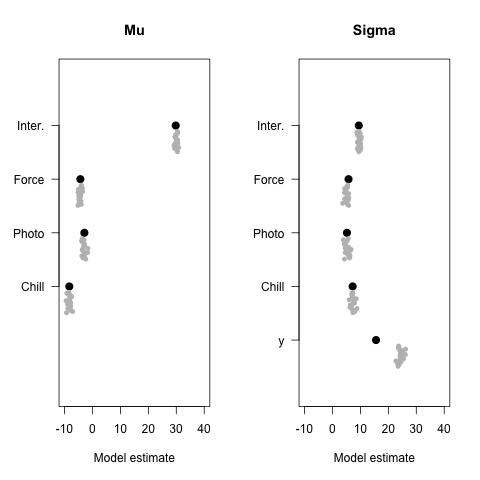
\includegraphics[width=0.9\textwidth]{..//..//..//..//analyses/bb_analysis/figures/measerrcomp.png}
\caption{Comparison of main budburst model estimates (black circles) to estimates from models that incorporate estimated measurement error (gray circles) for the main effects in our budburst model: $\mu_{\alpha}$ (`Interc.' for intercept), $\mu_{forcing}$ (`Force'), $\mu_{photoperiod}$ (`Photo'),and $\mu_{chilling}$ (`Chill'), as well as their associated $\sigma$ s ($\sigma_{\alpha}$, $\sigma_{forcing}$, $\sigma_{photoperiod}$, $\sigma_{chilling}$) and error ($\sigma_{y}$). We show means from the posterior distribution for Mus ($\mu$) in the left panel and Sigmas ($\sigma$) in the right panel.}
\label{fig:trtmap}
\end{figure}


\emph{4. Chilling and forcing time: I apologise if I have overlooked this but I still cannot find in the
methods or main text a clear statement of the dates over which chilling units (and forcing
units) were calculated. Figure 1 is helpful but does not include a specific statement about
timing. If timings are idiosyncratic to each study this should be made clear and it would be
really helpful to have a figure that shows for each study the time period of chilling and forcing.
This would also help the reader to evaluate whether the `chilling' metric is distinct from
forcing.}\\

Again, we apologize as we suspect this concern may be related to a lack of clarity on our meta-analysis focusing on short-term experiments that manipulate temperature and/or photoperiod, which we have attempted to clarify throughout the manuscript (see reply to 1. above for more details). As these are short-term experiments there is no consistent temporal window of when chilling was applied. We now mention that treatments vary by study early on in the caption to Fig. 1 and in the main text (see \lr{heatmap}), where we reference a heatmap figure that shows the treatments we have via our meta-analysis.

The length of time that chilling treatments were applied (as well as the temperature of these treatments) varied across experiments: chilling treatments from 1 to 182 days in duration (mean = 71.4 days) and temperatures ranged from  0 to 16 \degree C (mean = 4.4\degree C). The predictor variable ``chilling'' in our model is derived by applying standard chilling calculations to estimate the amount of chilling applied in these chilling treatments (we use both Utah units and Chill Portions in separate models, to compare the effect of using different chilling metrics). The predictor variable ``forcing'' is simply the forcing temperature applied; this also varied across experiments. To clarify this, we have also added the following to the legend of Figure 1: ``Across 72 studies examined, we found treatments varied uniquely for each study, but some were more common than others, see Fig. S3: chilling treatments averaged 71.4 days (range: 1-182 days) at an average temperature of 4.4 \degree C (range: 0-16 \degree C), forcing treatments averaged 15.7 \degree C (range: 5 to 32 \degree C).''

More detailed information, e.g., the temperatures and durations for forcing and chilling in each study can be found in the OSPREE database, which will be publicly available upon publication via the Knowledge Network for Biodiversity (part of DataONE, which should make these data discoverable through multiple portals). \\

\emph{5. Random regression covariances. In the random slopes model it looks as though the variance in
slopes across species for one driver is fitted as being independent of the variance across other
drivers. I think the covariances between these random slopes and the with the random
intercept should be estimated i.e. estimate a 4 x 4 covariance matrix (alphasp, betaforcing,
betaphotoperiod, betachilling).}\\

The reviewer is correct about our model formulation: we did not originally include these covariances. The use of this type of covariance matrix is generally considered a modelling choice \citep{gelman2006}, unless there are strong covariances, in which case a covariance matrix should definitely be included or the model re-formulated to better address the reasons for such covariances.  Our review of our models strongly suggested we were not missing any critical covariances. Based on the reviewer's request, we have added a covariance matrix to our main model to allow random slopes and intercepts to covary. The estimates from this new model are similar to those from our main model (e.g., 50\% credible intervals overlap). Please see table below, which compares model estimates from the two models below; we show the correlation matrix for species-level intercepts and slopes below. 

Table comparing model estimates from main model (e.g., Figure 2 in the main text, Figure S4 in the Supplemental Materials) to estimates from a model that includes a covariance matrix for species-level intercepts and slopes (i.e., random effects), with 95\% uncertainty intervals in parentheses:

% latex table generated in R 3.6.0 by xtable 1.8-4 package
% Thu Apr 16 23:23:19 2020
\begingroup\footnotesize
\begin{tabular}{|p{0.10\textwidth}|p{0.25\textwidth}|p{0.25\textwidth}|}
  \hline
 & main model & main model, with correlation matrix \\ 
  \hline
$\mu_{\alpha}$ & 29.87 (26.43, 33.41) & 29.67 (26.08, 33.05) \\ 
  $\mu_{forcing}$ & -4.35 (-6.52, -2.11) & -4.35 (-6.66, -2) \\ 
  $\mu_{photoperiod}$ & -2.92 (-5.38, -0.46) & -3.08 (-5.34, -0.87) \\ 
  $\mu_{chilling}$ & -8.36 (-11.41, -5.28) & -7.62 (-10.89, -4.42) \\ 
   \hline
\end{tabular}
\endgroup
\\ 
\\Correlation matrix for species-level intercepts and slopes (i.e., random effects):

% latex table generated in R 3.6.0 by xtable 1.8-4 package
% Thu Apr 16 23:23:19 2020
\begingroup\footnotesize
\begin{tabular}{|p{0.10\textwidth}|p{0.1\textwidth}p{0.1\textwidth}p{0.1\textwidth}p{0.1\textwidth}|}
  \hline
 & $\alpha_{sp}}$ & $\beta_{forcing_{sp}}$ & $\beta_{photoperiod_{sp}}$ & $\beta_{chilling_{sp}}$ \\ 
  \hline
$\alpha_{sp}}$ & 1.00 & 0.05 & -0.52 & -0.49 \\ 
  $\beta_{forcing_{sp}}$ & 0.05 & 1.00 & -0.30 & -0.00 \\ 
  $\beta_{photoperiod_{sp}}$ & -0.52 & -0.30 & 1.00 & 0.30 \\ 
  $\beta_{chilling_{sp}}$ & -0.49 & -0.00 & 0.30 & 1.00 \\ 
   \hline
\end{tabular}
\endgroup
\\ 

\par \emph{Minor comments}\\

\emph{Line 26. Insert ``forcing'' before temperature.}\\

We have made this change.\\ 

\emph{Line 107. I'm not convinced that it is often found to be the most important cue? it may be highly
dependent on how you define importance. If importance is defined as it's influence on year to year
variation then in the UK we find chilling to be a less important cue than forcing --see fig 1 in Roberts et
al.}\\

We agree with the reviewer, as we say in the abstract (see \lr{unifydebateend}), ``in current environmental conditions the dominant signal of climate change is from increased forcing,'' and we have worked to clarify our methods throughout (see reply to 1. above for more details). We have also adjusted the text to further clarify our meaning by adding additional citations and clarifying that we refer to experiments, see \lr{eeXstart}-\lr{eeXend}:
\begin{quote}
This has not been widely suggested previously, perhaps because little experimental work has directly manipulated chilling, and the few studies that have were designed to compare chilling versus photoperiod effects \emph{\citep[e.g.,][]{zohner2016,Basler:2014aa,Caffarra:2011qf,Laube:2014a}}, not chilling versus forcing effects. Process-based phenological models, however, that explicitly model chilling often find this cue to be most critical \emph{\citep[e.g.,][]{gauzere2019,Laube:2014a,Heide:2005aa}}.
\end{quote}
We now also cite \citet{roberts2015} on \lr{addedroberts}.\\

\emph{Last paragraph of methods: The start date of GDD models does not have to be specified by the
researcher, it can be estimated from the data.}\\

We thank the reviewer for pointing this out; estimating a start date for GDD \citep[as done in][]{roberts2015} may be a useful approach for many questions. For this aspect of the methods, the goal was to examine potential statistical artifacts in estimating changes in forcing sensitivity. To evaluate this potential, we chose a specific start and end date because this simplification allowed for a more straightforward understanding of the potential effects of statistical artifacts.\\

 \emph{Table S2. Are the window open and closed in ordinal days? I'm also skeptical as to the informativeness of fitting a sliding window to just 10 years of data.}\\

Yes, the units for `Windows Open' and `Window closed' in Table S2 are in ordinal days. We thank the reviewer for pointing out this lack of clarity and now define this in the table legend. To do this analysis, we followed the methods in \citet{simmonds2019}, the reference suggested by the reviewer in the previous version. We were happy to incorporate this and feel it has strengthened our manuscript. Additional sliding window analyses may be interesting, and we think would be an excellent topic for a paper focused on sliding-window methods, which are designed for observational data. Our manuscript is focused on short-term experiments, which cannot easily be used with the sliding window approach---we have worked to clarify our methods now (see reply to 1. above for more details).\\

 \emph{Signed}\\
 \emph{Ally Phillimore}

 \emph{(I sign all of my reviews)}

 \emph{References}

\emph{Roberts AMI, Tansey C, Smithers RJ, Phillimore AB (2015) Predicting a change in the order of spring
phenology in temperate forests. Global change biology, 7, 2603-2611.}

 \emph{Van De Pol M, Wright J (2009) A simple method for distinguishing within- versus between-subject effects
using mixed models. Animal Behaviour, 77, 753-758.}\\
\\ 

{\bf Reviewer \#2 (Remarks to the Author):}\\

\emph{Thanks for the revision. The authors made a good response, and most of my concerns were responded. As I pointed before, this is an interesting study in quantifying the relative importance among the most important 3 cues in spring phenology, and thus be valuable for global change ecology studies. }\\


\emph{However, I still not fully convinced the chilling effect overweight forcing and photoperiod. Could the uncertainty in the experimental studies be quantified in the hierarchical Bayesian model? The experimental studies were theologically designed to estimate one cue effect, but interactive effect with other cues were actually not excluded, thus the solely effect of one cues might be overestimated.}\\ 

We appreciate the reviewer's concern, as this is one we had ourselves when we saw the results and we have worked to interrogate our model fully (we present six additional versions of our primary statistical model in the Supplemental Materials, Tables S5-S7, for this very reason). We have addressed this in several ways. We now reference a heatmap figure that shows the treatments we have via our meta-analysis in  caption to Fig. 1 and in the main text (see \lr{heatmap}, this figure shows we do have substantial variation across the three factors, as is critical for a robust model). Additionally, to interrogate whether our model estimates may be biased by studies that do not include interactions between multiple cues, we fit our main budburst model to a new subset of experiments: only those that tested at least two interactions between cues. We found that our model estimates did not qualitatively change when fitting the model to this subset of data, and have added a new table to our Supplemental Materials (Table S7).\\
%  also relates to Rev 1 interest in uncertainty

\emph{In addition, the authors argued that the decreased winter temperature during hiatus is not necessarily resulting an increase in chilling, but warming winter reduced chilling as most studied reported, thus both warming and cooling winter would reduce chilling? This is tricky, and may overestimate the chilling effect.}\\

We believe we may agree with the reviewer, but we did not clarify well enough in our previous drafts when we were we referring to chilling in short-term experiments that controlled temperature and photoperiod versus long-term climate data from Central Europe. In response to this Reviewer and Reviewer 1, we have worked to clarify this throughout our manuscript. In particular we have reduced our use of the phrase `controlled environment studies' and more often refer to `experiments with controlled temperature and/or photoperiod conditions.' This occurs throughout the paper, including in the abstract (\lr{ee1}), where instead of referring to `controlled environment studies' we now call them experiments, and mention again `controlled conditions'), also please see \lr{ee2start}-\lr{ee2end} and \lr{ee3start}-\lr{ee3end} and \lr{ee4}, \lr{ee5} and \lr{ee6}, \lr{ee7},\lr{ee8}, \lr{ee9}. We additionally edited all figure captions for clarity. \\

\emph{Anyway, this is valuable investigation in quantifying the environmental effects on spring budbreak spring, but the reliability is still need further estimation.}\\

We completely agree further work is needed and have aimed to stress this in our manuscript (see \lr{R2_1}, \lr{R2_2}, for example).\\

{\bf Reviewer \#3 (Remarks to the Author):}\\

\emph{The authors have done a great job in revising the manuscript. The additional analyses and figures they present have clarified the points raised in the previous review round and greatly improved the overall presentation of the data. I agree with all the conclusions and have no more comments.}\\

We thank the reviewer for the time spent reviewing our manuscript, and hope it will encourage more work on separating out chilling and forcing effects. \\

\bibliography{..//..//..//..//refs/ospreebibplus}

%%%%%%%%%%%%%%%%%%%%%%%%%%%%%%%%%%%%%%%%
\end{document}
%%%%%%%%%%%%%%%%%%%%%%%%%%%%%%%%%%%%%%%%
